\documentclass[11pt,a4paper]{article}
\usepackage[margin=1in]{geometry}
\usepackage{tikz}
\usetikzlibrary{arrows.meta,positioning,fit,calc,shapes.geometric}
\usepackage{titlesec}
\titleformat{\section}{\Large\bfseries}{}{0pt}{}
\title{AutoNexa System Architecture Block Diagrams}
\author{}
\date{March 29, 2026}

\tikzset{
  block/.style={draw, rounded corners, minimum height=10mm, minimum width=25mm, align=center, fill=blue!8},
  hw/.style={draw, rounded corners, minimum height=10mm, minimum width=25mm, align=center, fill=orange!12},
  sw/.style={draw, rounded corners, minimum height=10mm, minimum width=25mm, align=center, fill=green!10},
  safety/.style={draw, rounded corners, minimum height=10mm, minimum width=25mm, align=center, fill=red!10},
  io/.style={draw, rounded corners, minimum height=10mm, minimum width=25mm, align=center, fill=purple!10},
  line/.style={-Latex, thick},
  dashedline/.style={-Latex, thick, dashed}
}

\begin{document}
\maketitle

\section*{1) Overall System Block Diagram}
\begin{center}
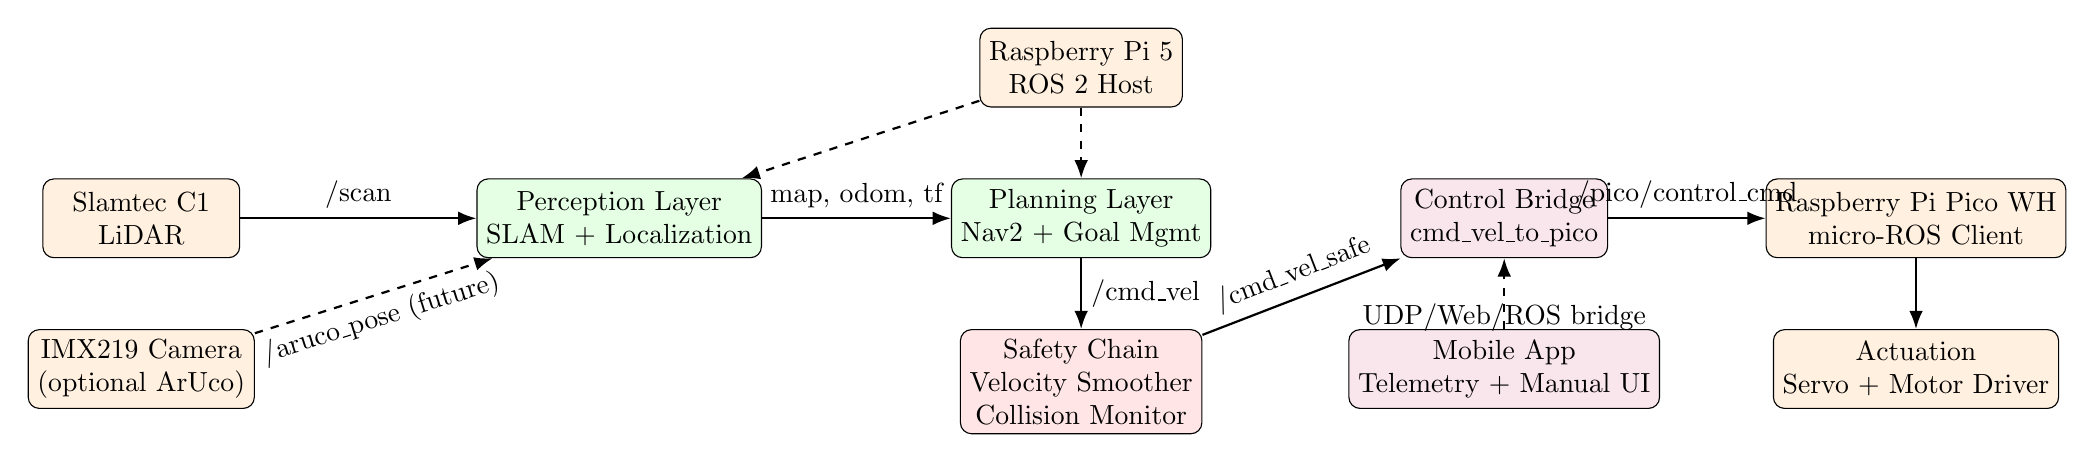
\begin{tikzpicture}[node distance=9mm and 10mm]
  \node[hw] (lidar) {Slamtec C1\\LiDAR};
  \node[hw, below=of lidar] (camera) {IMX219 Camera\\(optional ArUco)};
  \node[sw, right=30mm of lidar] (perception) {Perception Layer\\SLAM + Localization};

  \node[sw, right=24mm of perception] (nav2) {Planning Layer\\Nav2 + Goal Mgmt};
  \node[safety, below=of nav2] (safetychain) {Safety Chain\\Velocity Smoother\\Collision Monitor};

  \node[io, right=24mm of nav2] (bridge) {Control Bridge\\cmd\_vel\_to\_pico};
  \node[hw, right=20mm of bridge] (pico) {Raspberry Pi Pico WH\\micro-ROS Client};
  \node[hw, below=of pico] (act) {Actuation\\Servo + Motor Driver};

  \node[hw, above=of nav2] (rpi5) {Raspberry Pi 5\\ROS 2 Host};
  \node[io, below=of bridge] (mobile) {Mobile App\\Telemetry + Manual UI};

  \draw[line] (lidar) -- node[above,sloped]{/scan} (perception);
  \draw[dashedline] (camera) -- node[below,sloped]{/aruco\_pose (future)} (perception);
  \draw[line] (perception) -- node[above]{map, odom, tf} (nav2);
  \draw[line] (nav2) -- node[right]{/cmd\_vel} (safetychain);
  \draw[line] (safetychain) -- node[above,sloped]{/cmd\_vel\_safe} (bridge);
  \draw[line] (bridge) -- node[above]{/pico/control\_cmd} (pico);
  \draw[line] (pico) -- (act);

  \draw[dashedline] (rpi5) -- (perception);
  \draw[dashedline] (rpi5) -- (nav2);
  \draw[dashedline] (mobile) -- node[below]{UDP/Web/ROS bridge} (bridge);
\end{tikzpicture}
\end{center}

\section*{2) Perception Subsystem}
\begin{center}
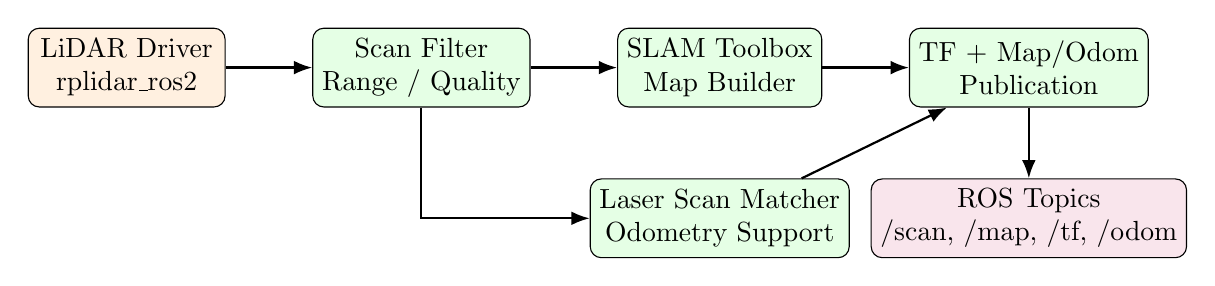
\begin{tikzpicture}[node distance=9mm and 11mm]
  \node[hw] (scan) {LiDAR Driver\\rplidar\_ros2};
  \node[sw, right=of scan] (prefilter) {Scan Filter\\Range / Quality};
  \node[sw, right=of prefilter] (slam) {SLAM Toolbox\\Map Builder};
  \node[sw, below=of slam] (matcher) {Laser Scan Matcher\\Odometry Support};
  \node[sw, right=of slam] (tfpub) {TF + Map/Odom\\Publication};
  \node[io, below=of tfpub] (topics) {ROS Topics\\/scan, /map, /tf, /odom};

  \draw[line] (scan) -- (prefilter);
  \draw[line] (prefilter) -- (slam);
  \draw[line] (prefilter) |- (matcher);
  \draw[line] (slam) -- (tfpub);
  \draw[line] (matcher) -- (tfpub);
  \draw[line] (tfpub) -- (topics);
\end{tikzpicture}
\end{center}

\section*{3) Navigation Subsystem}
\begin{center}
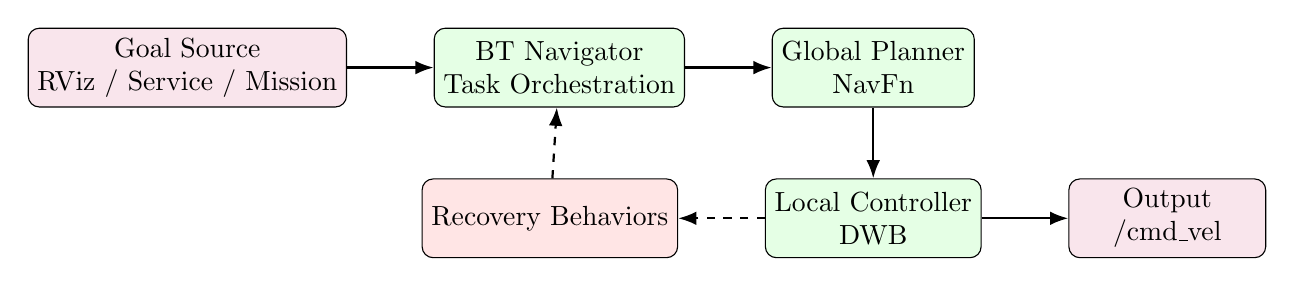
\begin{tikzpicture}[node distance=9mm and 11mm]
  \node[io] (goal) {Goal Source\\RViz / Service / Mission};
  \node[sw, right=of goal] (bt) {BT Navigator\\Task Orchestration};
  \node[sw, right=of bt] (planner) {Global Planner\\NavFn};
  \node[sw, below=of planner] (controller) {Local Controller\\DWB};
  \node[safety, left=of controller] (recoveries) {Recovery Behaviors};
  \node[io, right=of controller] (cmd) {Output\\/cmd\_vel};

  \draw[line] (goal) -- (bt);
  \draw[line] (bt) -- (planner);
  \draw[line] (planner) -- (controller);
  \draw[line] (controller) -- (cmd);
  \draw[dashedline] (controller) -- (recoveries);
  \draw[dashedline] (recoveries) -- (bt);
\end{tikzpicture}
\end{center}

\section*{4) Control + Safety Subsystem}
\begin{center}
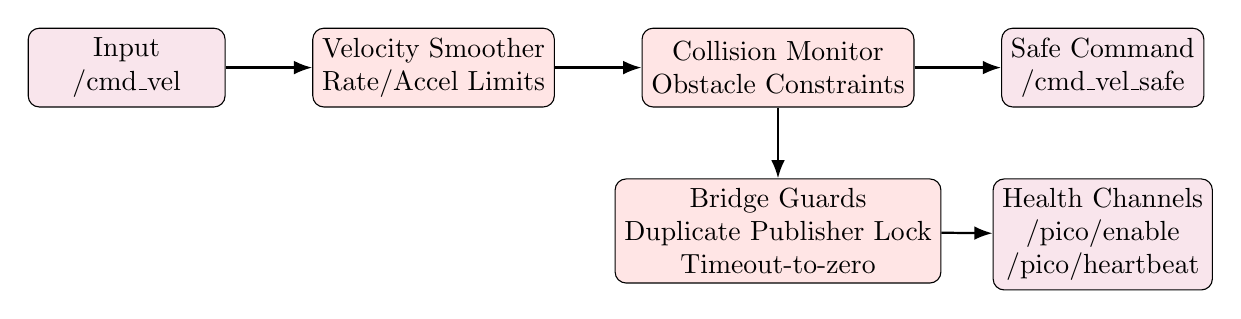
\begin{tikzpicture}[node distance=9mm and 11mm]
  \node[io] (in) {Input\\/cmd\_vel};
  \node[safety, right=of in] (smoother) {Velocity Smoother\\Rate/Accel Limits};
  \node[safety, right=of smoother] (collision) {Collision Monitor\\Obstacle Constraints};
  \node[safety, below=of collision] (arb) {Bridge Guards\\Duplicate Publisher Lock\\Timeout-to-zero};
  \node[io, right=of collision] (safeout) {Safe Command\\/cmd\_vel\_safe};
  \node[io, below=of safeout] (health) {Health Channels\\/pico/enable\\/pico/heartbeat};

  \draw[line] (in) -- (smoother);
  \draw[line] (smoother) -- (collision);
  \draw[line] (collision) -- (safeout);
  \draw[line] (collision) -- (arb);
  \draw[line] (arb) -- (health);
\end{tikzpicture}
\end{center}

\section*{5) Embedded (Pico Firmware) Subsystem}
\begin{center}
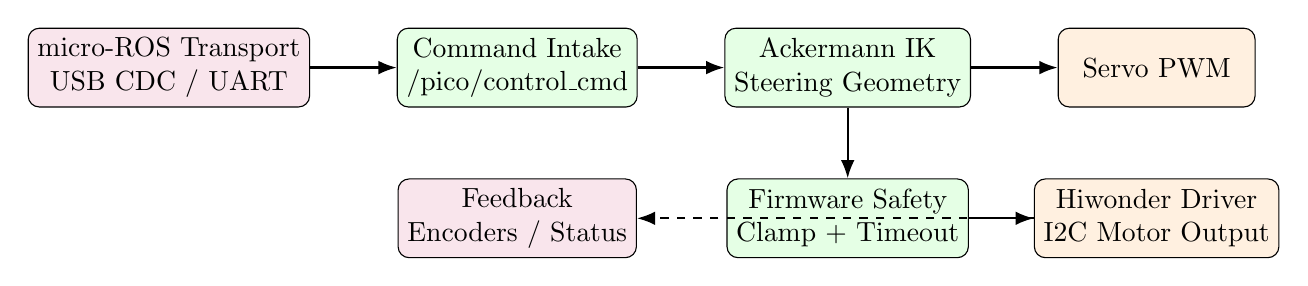
\begin{tikzpicture}[node distance=9mm and 11mm]
  \node[io] (uros) {micro-ROS Transport\\USB CDC / UART};
  \node[sw, right=of uros] (cmdrx) {Command Intake\\/pico/control\_cmd};
  \node[sw, right=of cmdrx] (ack) {Ackermann IK\\Steering Geometry};
  \node[sw, below=of ack] (safetyfw) {Firmware Safety\\Clamp + Timeout};
  \node[hw, right=of ack] (servo) {Servo PWM};
  \node[hw, below=of servo] (motor) {Hiwonder Driver\\I2C Motor Output};
  \node[io, below=of cmdrx] (fb) {Feedback\\Encoders / Status};

  \draw[line] (uros) -- (cmdrx);
  \draw[line] (cmdrx) -- (ack);
  \draw[line] (ack) -- (servo);
  \draw[line] (ack) -- (safetyfw);
  \draw[line] (safetyfw) -- (motor);
  \draw[dashedline] (motor) -- (fb);
\end{tikzpicture}
\end{center}

\section*{6) Communications Matrix (Subsystem Interfaces)}
\begin{center}
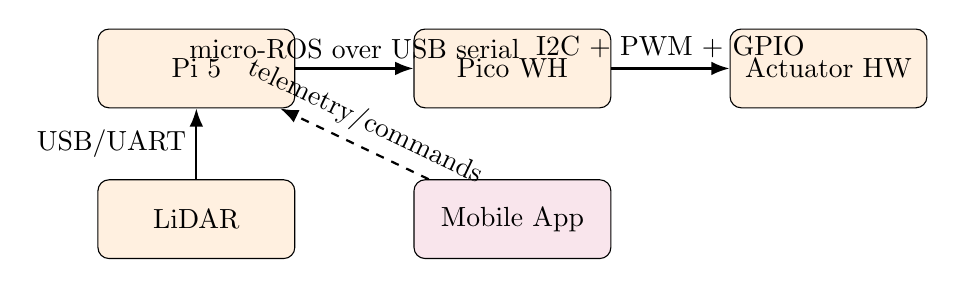
\begin{tikzpicture}[node distance=9mm and 15mm]
  \node[hw] (pi) {Pi 5};
  \node[hw, right=of pi] (pico2) {Pico WH};
  \node[hw, right=of pico2] (drivers) {Actuator HW};
  \node[hw, below=of pi] (lidar2) {LiDAR};
  \node[io, below=of pico2] (app) {Mobile App};

  \draw[line] (lidar2) -- node[left]{USB/UART} (pi);
  \draw[line] (pi) -- node[above]{micro-ROS over USB serial} (pico2);
  \draw[line] (pico2) -- node[above]{I2C + PWM + GPIO} (drivers);
  \draw[dashedline] (app) -- node[above,sloped]{telemetry/commands} (pi);
\end{tikzpicture}
\end{center}

\end{document}
